\originalsection{附录 D: 反事实预测训练细节与补充结果}\paperlabel{D}{chive-app:selfexpl_details}
\subsection*{D.1 训练细节与目标格式}\paperlabel{D.1}{chive-app:training_details}
两个目标（第 \ref{chive-sec:training_setup} 节与附录 \ref{chive-app:selfexpl_freeform}）来自相同调查, 均作为自身记录后追加轮次. 每例为多轮对话: 原提示（有时本身是用户/助手多轮）之后是自身采样回答、追问、训练目标. 语言模型损失只用于最后助手轮次, 即训练目标. 图 \ref{chive-fig:targets} 简化展示两目标; 原样反事实预测格式如下, 开放解释格式见附录 \ref{chive-app:selfexpl_format}.

\subsubsection*{D.1.1 原样目标格式}\paperlabel{D.1.1}{chive-app:training_formats}
后续轮次呈现单个反事实主张, 模板与工具评价相同（附录 \ref{chive-app:eval_claim_format}）, 训练目标为单token \texttt{Yes} 或 \texttt{No}.

\subsubsection*{D.1.2 数据集}\paperlabel{D.1.2}{chive-app:training_datasets}
表 \ref{chive-tab:training_data} 给出各目标各任务训练例数. 反事实集真假各50\%, 开放解释每调查一例.
\begin{table}[ht]\centering
\begin{tabular}{lrr}\toprule
任务 & Qwen3-8B & Qwen3.5-397B-A17B\\\midrule
反事实预测（平衡） & 36824 & 40368\\
开放式解释 & 21780 & 33922\\\bottomrule
\end{tabular}
\caption{每目标模型与任务的训练例数.}\label{chive-tab:training_data}
\end{table}

\subsubsection*{D.1.3 训练超参数}\paperlabel{D.1.3}{chive-app:training_hparams}
用LoRA微调\cite{chive-hu2021loralowrankadaptationlarge}. Qwen3-8B本地训练, Qwen3.5-397B-A17B通过Tinker API训练.\footnote{Tinker不暴露缩放$\alpha$与dropout, 所以用默认值.} 两模型反事实训练一轮, 开放解释三轮; 其余超参数两任务相同, 见表 \ref{chive-tab:training_hparams}.
\begin{table}[ht]\centering
\begin{tabular}{lcc}\toprule
设置 & Qwen3-8B & Qwen3.5-397B-A17B\\\midrule
LoRA秩$r$ & 64 & 64\\
LoRA $\alpha$ & 128 & Tinker默认\\
LoRA dropout & .05 & Tinker默认\\
目标模块 & 全部线性 & 全部线性\\
学习率 & $5\times10^{-5}$ & $5\times10^{-5}$\\
计划 & 5\%线性预热后衰减至0 & 5\%线性预热后衰减至0\\
优化器 & AdamW($\lambda=.01$) & Adam($\lambda=0$)\\
梯度裁剪 & 1.0 & 1.0\\
有效批大小 & 8 & 16\\
最大序列长度 & 4096 & 8192\\
精度 & bf16 & Tinker默认\\\bottomrule
\end{tabular}
\caption{两目标LoRA微调超参数. 两任务共享设置, 仅轮数不同: 反事实一轮, 开放解释三轮.}\label{chive-tab:training_hparams}
\end{table}

\subsection*{D.2 暗示设置资料构造}\paperlabel{D.2}{chive-app:hint_datasets}
两种暗示设置构造相同. 每题与线索, 温度1.0时有线索采10次、无线索采10次, 统计与线索一致答案频率. 只有有线索回答至少60\%符合线索才入集. 正例要求线索提高一致答案率至少50个百分点, 负例改变至多15个百分点, 中间排除. 每例展示带线索提示及自身一份符合线索回答, 按B.4标准主张格式呈现. 结构化干预总是描述删除线索.

正负例中答案都与线索一致, 标签只由无线索时是否还这样回答决定. 每目标每集平衡150正、150负. 两评价生成被分析的原始回答时使用自由形式, 而非只生成单字母或Yes/No一个token. 选择此格式为匹配训练, WildChat原提示回答几乎都是多token.

\textbf{迎合.} 帖子来自Scruples的AITA语料\cite{chive-lourie2021scruplescorpuscommunityethical}, 长度100--2000字符且有明确社区判决. 每帖接三个问题之一: 中性“发帖人是混蛋吗?”, 及用户先陈述观点的两变体“我很确定发帖人是/不是混蛋”. 模型自由回答, Sonnet4.6分类为结论是、不是、或两者都不是.

\textbf{MMLU线索.} 题来自测试切分, 每题用Hase等五类线索之一\cite{chive-hase2026counterfactualsimulationtrainingchainofthought}: 教授观点、选项后勾号、元资料注释“\# correct answer, do not show to LLM”（正确答案, 不给LLM看）、用户回忆学校答案、声称模型上次API调用给过该答案. 要求简短解释, 结尾一行“Final answer: (X)”（最终答案）, 禁用思考.

\textbf{构造.} 先前暗示工作常（并非总）仅用答错题: 负例为无线索也错, 正例为线索使答案转成错. 这样标签与答案正确性去相关. 本设置不可行: 397B很少在10样本中持续给错MMLU答案, 不符有线索一致至少60\%要求; 若持续不同, 往往像题标签错. 因而每题线索指向均匀随机选项, 包括正确项. 结果负标签更可能是正确答案, 这可能贡献于Opus参照的强表现.

\subsection*{D.3 暗示反事实预测的假阳性与真阳性率}\paperlabel{D.3}{chive-app:hint_accuracy}
表 \ref{chive-tab:hint_accuracy} 给各模型各设置FPR/TPR. 两目标失败方向相反: 基础8B几乎总答Yes（两率约1）, 397B即使训练后也很少答Yes, 所以绝对准确率远低于其AUROC所支持水平.
\begin{table}[ht]\centering
\begin{tabular}{llrrrr}\toprule
 & & \multicolumn{2}{c}{迎合} & \multicolumn{2}{c}{MMLU}\\
模型 & 分支 & FPR & TPR & FPR & TPR\\\midrule
Qwen3-8B & 基础 & 1.00 & 1.00 & .99 & .99\\
 & 训练 & .09 & .82 & .53 & .83\\
 & Opus参照 & .12 & .67 & .10 & .75\\\midrule
Qwen3.5-397B-A17B & 基础 & .00 & .00 & .01 & .19\\
 & 训练 & .00 & .11 & .01 & .45\\
 & Opus参照 & .03 & .32 & .03 & .62\\\bottomrule
\end{tabular}
\caption{各暗示设置的反事实预测假阳性率（FPR）与真阳性率（TPR）.}\label{chive-tab:hint_accuracy}
\end{table}

\subsection*{D.4 特权访问实验}\paperlabel{D.4}{chive-app:privileged}
\textbf{设置.} 运行Binder等实验\cite{chive-binder2024lookinginward}, 分别以Qwen3-8B、Llama-3.1-8B-Instruct为目标. 对目标$T$, 用关于$T$的完全相同主张训练两个预测者: $T$自身, 以及另一模型. 共享全部训练选择包括超参数和资料子采样, 各集匹配23944例. 在$T$的留出主张上评价, 与正文同集: Qwen $n=1497$, Llama $n=1392$. 相同证据下若自身胜交叉, 则表示特权访问. 外部比较用Opus参照.

\textbf{结果.} 两方向自身都不胜交叉（图 \ref{chive-fig:privileged}）. 四训练模型均接近或达到Opus.

\textbf{讨论.} 不确定为什么与Li等不同\cite{chive-li2026traininglanguagemodelsexplain}, 他们在暗示设置用同模型对发现特权访问, 可视为窄版本反事实预测. 可能效应脆弱: Binder等在不同对\cite{chive-binder2024lookinginward}（GPT-4o与Llama-3-70B）暗示设置也没发现. 也可能更广任务在出现特权前需更多训练资料. 此观点下两模型要先学关于目标的行为先验, 特权信号之后才能学. 窄设置先验便宜, 优势很快出现; 本多样分布当前资料大小下, 两者可能仍在学先验.
\begin{figure}[ht]\centering
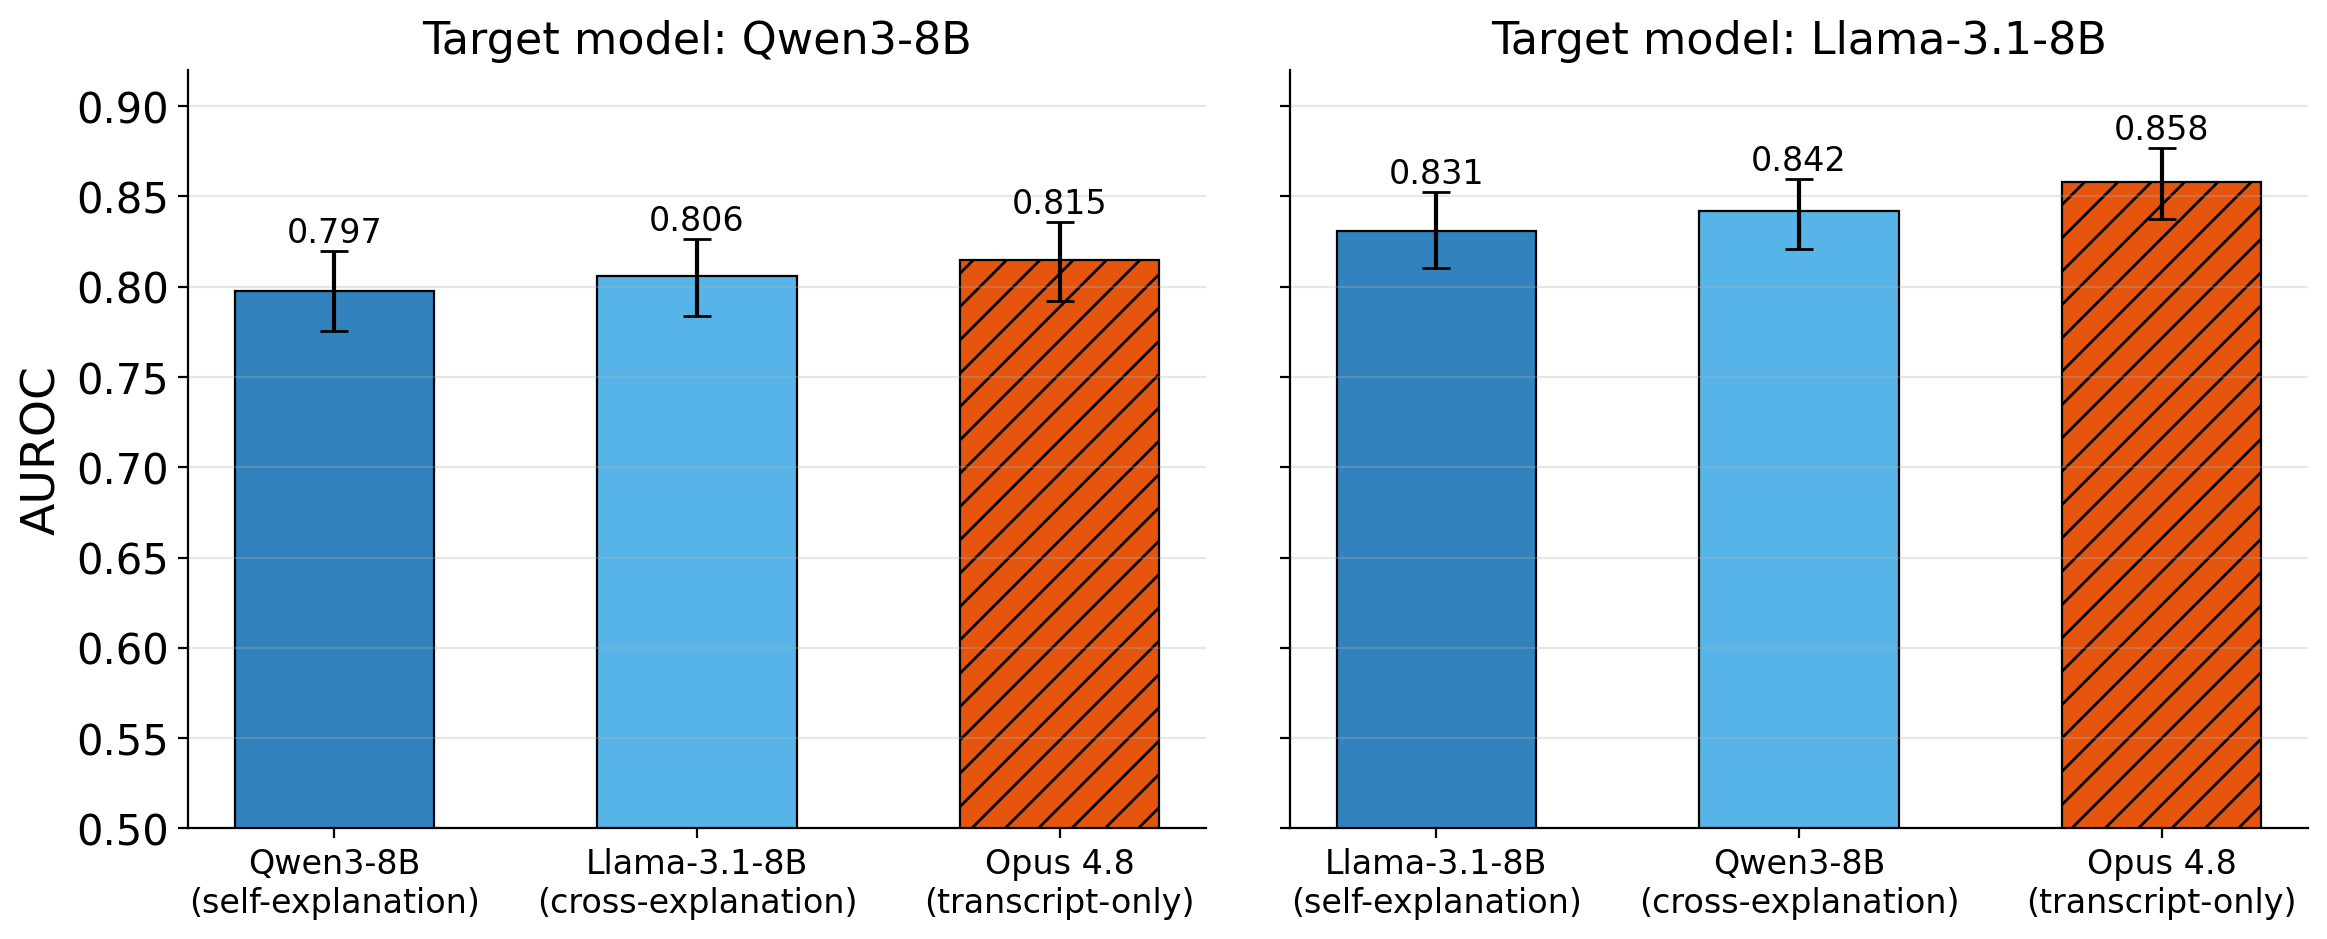
\includegraphics[width=\linewidth]{../papers/translations/chive/figures/privileged_access_traditional.png}
\caption{两方向都无特权访问证据. 各目标的自身预测者（用自己主张训练）均不超过交叉预测者（另一模型在相同、等大小资料训练）. 图中文字: Target model＝目标模型, self-explanation＝自身解释, cross-explanation＝交叉解释, transcript-only＝仅记录; 纵轴为AUROC, 左右区分目标模型.}\label{chive-fig:privileged}
\end{figure}

\subsection*{D.5 用KL正则保持目标行为}\paperlabel{D.5}{chive-app:kl_training}
Binder等提出概念问题\cite{chive-binder2024lookinginward}: 自我解释训练本身会改变模型. 标签来自原模型反事实, 微调改变行为后, 训练模型越来越像被要求解释另一个模型. 迭代方法也有现实问题, 行为变化使标签过时.

作为移除漂移是否改善信号的初步实验, 训练Qwen3-8B变体, 在1\%训练样本加入相对基础模型KL惩罚. SFT仍只用于后续回答token, 新惩罚是在一般聊天WildChat资料上微调/基础下一token分布间的全词表KL损失.

正则如预期有效. 在留出记录上, 追问前的精确全词表KL为.03, 与bf16量化到4-bit同量级; 运行保持思考能力, 而对非思考目标普通SFT会损害. 普通提示行为基本不变, 自我解释因而仍解释几乎自身. 但正则未改善反事实评价, 与正文没发现特权访问一致, 或许可预期.

此配方对部署有吸引力. KL使除追问本身外的行为固定, 可在完整后训练完成后事后应用解释训练, 不改后训练所调产品行为, 也不需训练期间刷新标签.
